\chapter{Testy}
\section{Testy jednostkowe}
Projekt serwera testowany jest za pomocą testów jednostkowych z użyciem biblioteki MSTest. Aby testy mogły zostać uruchomione, niezbędne jest uruchomienie bazy danych MongoDB pod lokalnym adresem oraz domyślnym portem (27017). Testowane jest podstawowe połączenie z bazą danych oraz operacje na niej, a także serwisy: logowania, rejestracji, losowania hasła, tworzenia pokoju oraz wyliczania rankingu.

W sumie napisane zostały 44 testy jednostkowe, sprawdzające poprawność działania usług pod kątem nie tylko standardowego wywołania, ale też róznych sytuacji brzegowych, takich jak na przykład niepoprawne argumenty.

Konwencja nazewnictwa testów jest następująca: nazwaMetody{\_}warunki{\_}oczekiwanyRezultat.

W sprawnym pisaniu warunków asercji pomogła nam biblioteka FluentAssertions, dostępna jako paczka NuGet (http://www.fluentassertions.com/). Przykład jej użycia widać na rysunku \ref{fig:fluentassertions}.

\begin{figure}[htbp]
\centering
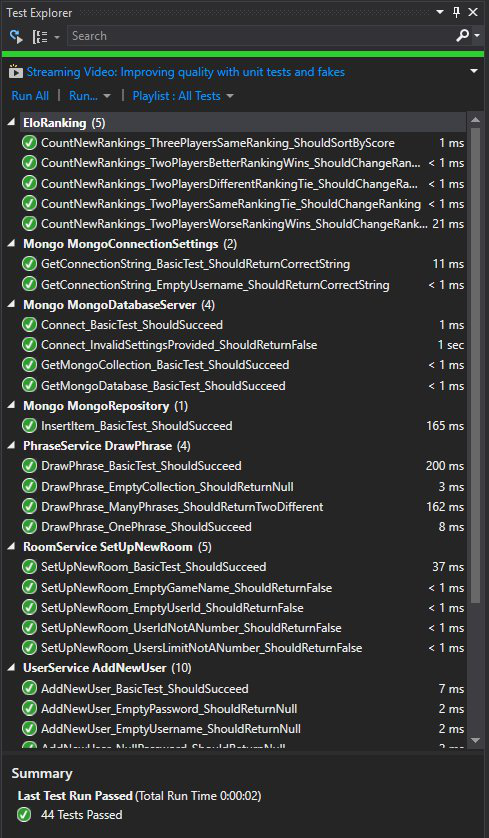
\includegraphics[width=0.5\textwidth]{UnitTests}
\caption{Wynik uruchomienia\\wszystkich testów jednostkowych.}
\label{fig:unittests}
\end{figure}

\begin{figure}[htbp]
\centering
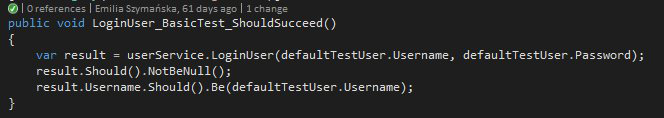
\includegraphics[width=\textwidth]{FluentAssertions}
\caption{Przykład asercji z użyciem biblioteki FluentAssertions.}
\label{fig:fluentassertions}
\end{figure}

\section{Testy integracyjne}
Pełne środowisko testowe składało się z następujących elementów:
\begin{itemize}
    \item Maszyna wirtualna stworzona na platformie Azure:
    \begin{itemize}
    \item System operacyjny: Windows Server 2012, x64
    \item Ilość rdzeni: 1 x 2.20 GHz
    \item Ilosć pamięci RAM: 1,75 GB
    \item Adres DNS: sculpicserver.cloudapp.net
    \end{itemize}
    z uruchomionymi instancjami MasterServera, serwera WCF oraz uruchamianymi w miarę potrzeb instancjami pokojów (Sculpic Hoster). Uruchomiona jest też baza danych MongoDB dostępna lokalnie pod domyślnym portem.
    \item Urządzenia mobilne:
    \begin{center}
    \begin{tabular}{|m{2cm}|m{3cm}|m{2cm}|m{3cm}|}
    \hline
    Rodzaj urządzenia & Model & Wielkość ekranu & Rozdzielczość ekranu \\ \hline \hline
    Smartfon & Sony Xperia P & 4’’ & 540 x 960 px \\ \hline
    Smartfon & Samsung Galaxy Note III & 5,7’’ & 1080 x 1920 px \\ \hline
    Smartfon & Samsung Galaxy S5 & 5,1’’ & 1080 x 1920 px \\ \hline
    Tablet & Samsung Galaxy Tab 2 & 10,1’’ & 1280 x 800 px \\ \hline
    \end{tabular}
    \end{center}
\end{itemize}

Na wszystkich wyżej wymienionych urządzeniach aplikacja działała poprawnie. Na każdym z nich została dokładnie sprawdzona cała funkcjonalność wraz z jednoczesnym prowadzeniem rozgrywki (w jednym pokoju). Poniżej zaprezentowane są zrzuty ekranu z urządzeń, na których można zaobserwować skalowalność interfejsu użytkownika:

\begin{figure}[htbp]
\centering
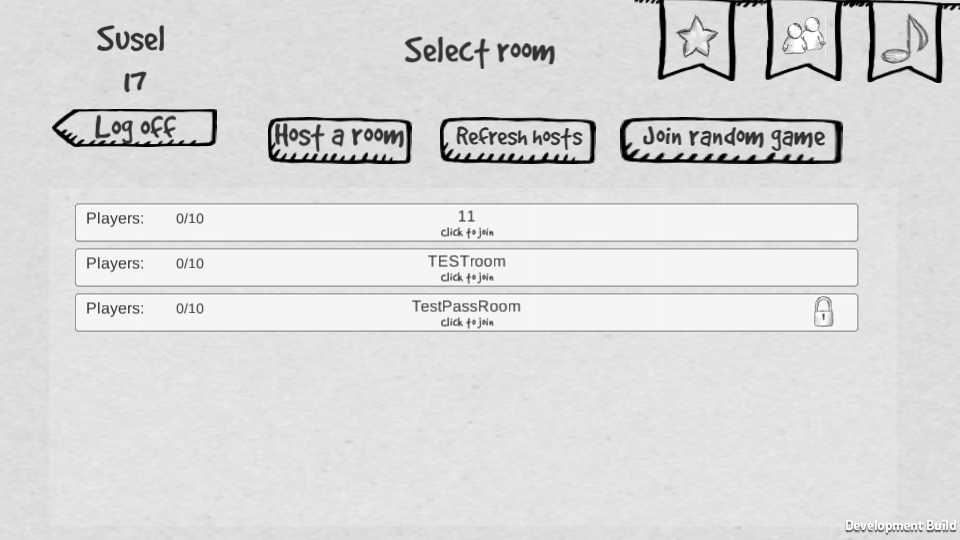
\includegraphics[width=\textwidth]{Screen1}
\caption{Zrzut ekranu z telefonu Sony Xperia P.}
\label{fig:screen1}
\end{figure}

\begin{figure}[htbp]
\centering
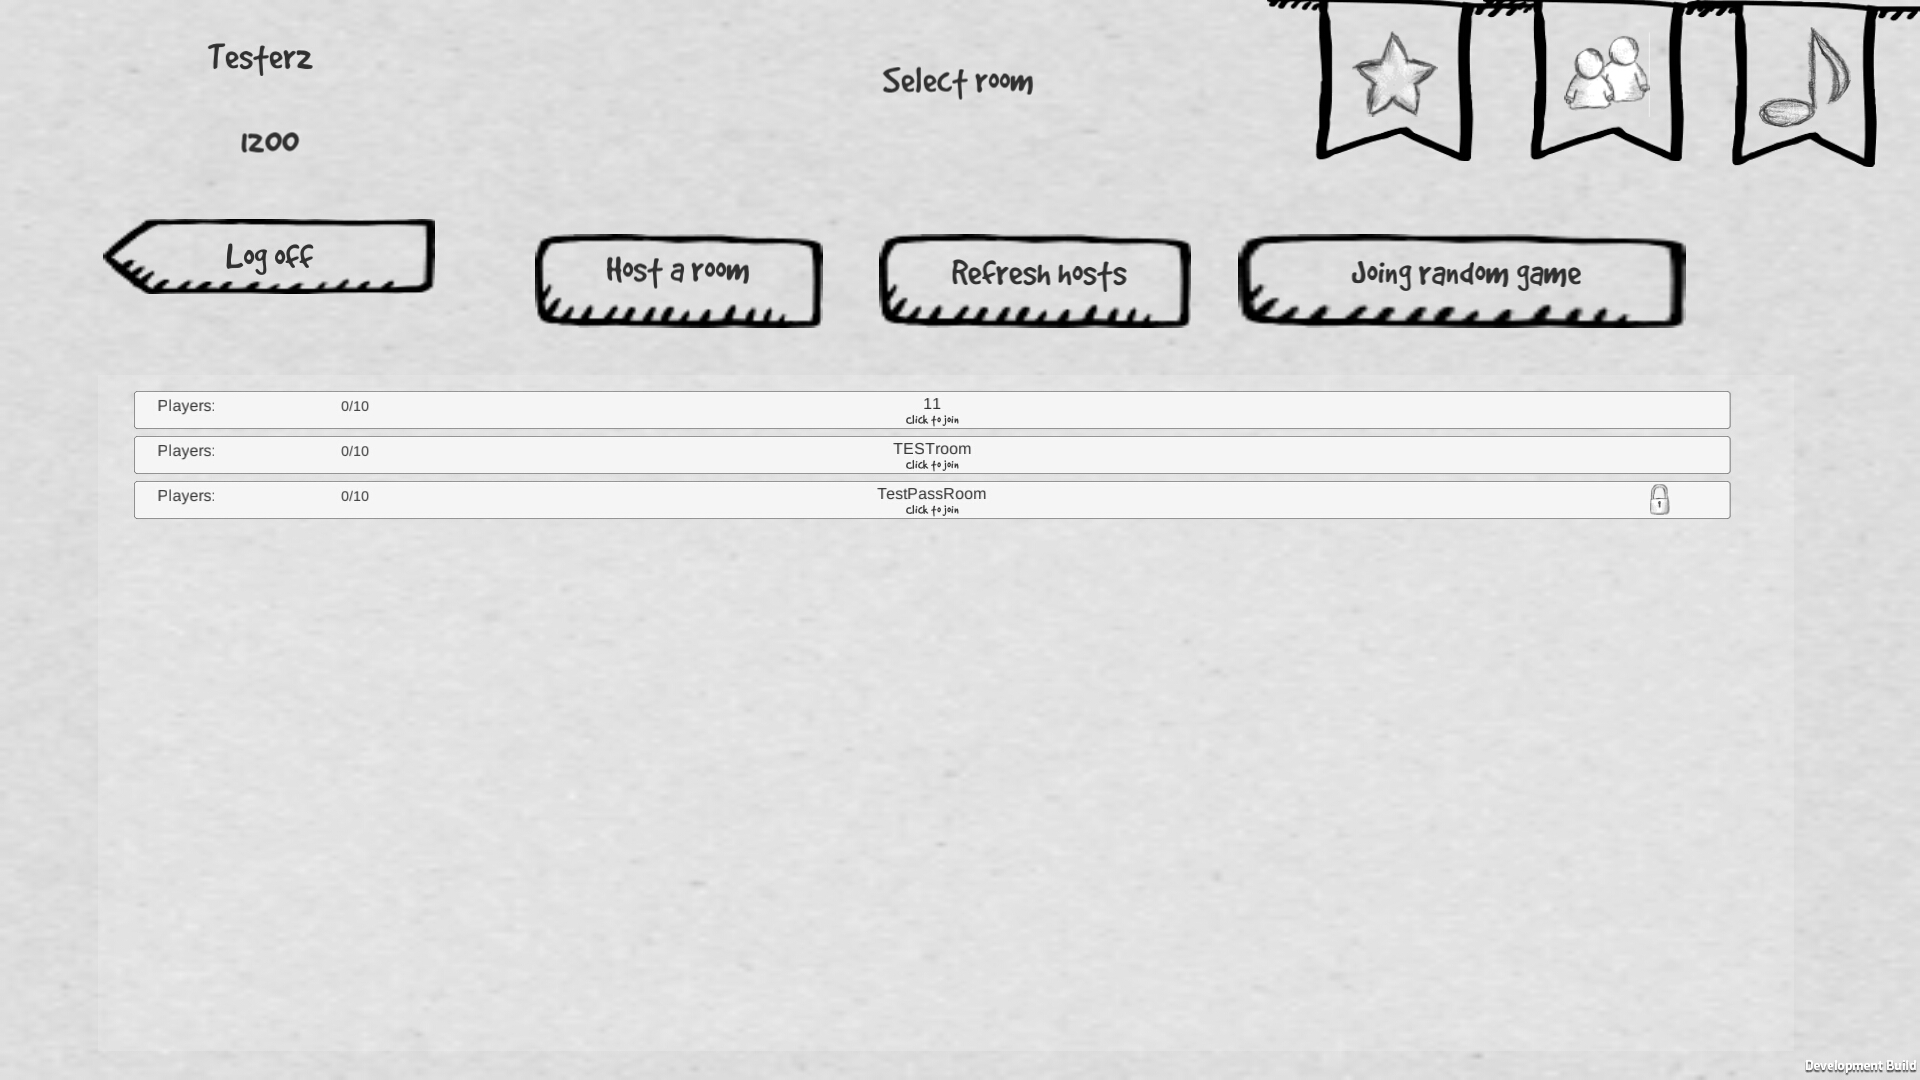
\includegraphics[width=\textwidth]{Screen2}
\caption{Zrzut ekranu z telefonu Galaxy Note III.}
\label{fig:screen2}
\end{figure}

\begin{figure}[htbp]
\centering
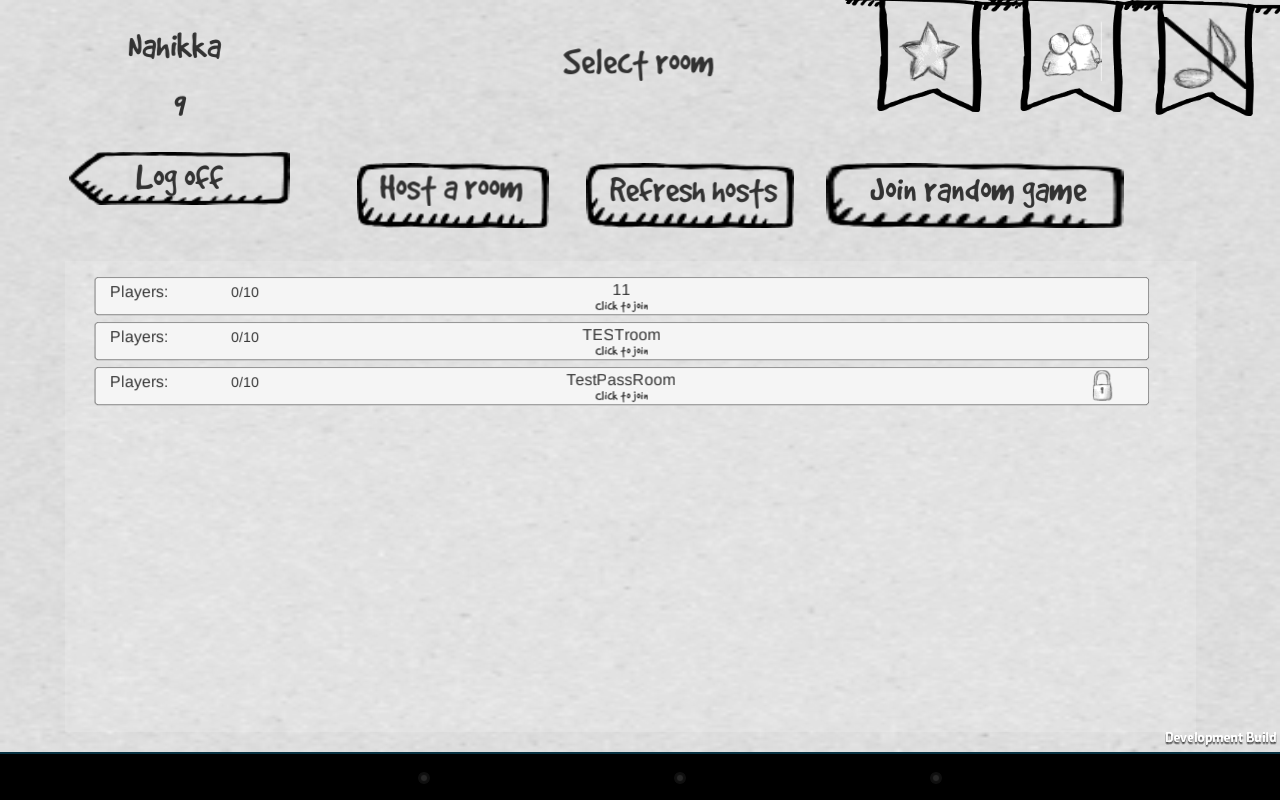
\includegraphics[width=\textwidth]{Screen3}
\caption{Zrzut ekranu z tabletu Galaxy Tab 2.}
\label{fig:screen3}
\end{figure}